
\tikzstyle{process} = [rectangle, fill=blue!20, minimum width=1.5cm, minimum height=0.8cm, text centered, draw=black]
\tikzstyle{arrow} = [thick,->,>=stealth]

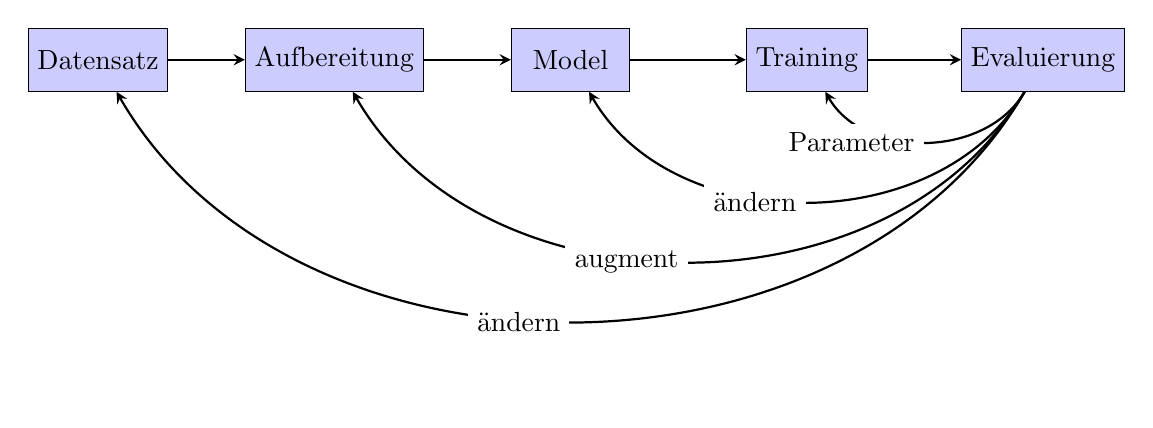
\begin{tikzpicture}[scale=0.4]

     \begin{scope}[node distance=3cm]

      \node (data)      [process]                   {Datensatz};
      \node (prep)      [process, right of=data]      {Aufbereitung};
      \node (model)      [process, right of=prep]      {Model};
      \node (train)      [process, right of=model]      {Training};
      \node (eval)      [process, right of=train]      {Evaluierung};

     \end{scope}

    \draw[arrow] (data) -- (prep);
    \draw[arrow] (prep) -- (model);
    \draw[arrow] (model) -- (train);
    \draw[arrow] (train) -- (eval);
    

  \draw[arrow] (eval) edge[bend left=60] node [left, fill=white!30] {ändern} (data);
  \draw[arrow] (eval) edge[bend left=60] node [left, fill=white!30] {augment} (prep);
  \draw[arrow] (eval) edge[bend left=60] node [left, fill=white!30] {ändern} (model);
  \draw[arrow] (eval) edge[bend left=60] node [left, fill=white!30] {Parameter} (train);

    
\end{tikzpicture}
